\documentclass[16pt]{beamer}
\usepackage[utf8]{inputenc}
\usepackage{media9}
\usepackage{amsmath}
\usepackage{amsfonts}
\usepackage{amssymb}
\usepackage{amsthm}
\usepackage{graphicx,epsfig}
 
% \usetheme{Madrid}
% \usecolortheme{beaver}

\usepackage{anyfontsize}
 
\begin{document}

\begin{frame}
	\fontsize{15}{7.2}\selectfont
	February 9, 1938
	\begin{figure}[H]
	\centering
	\includegraphics[width=0.7\textwidth]{images/goldengate.jpg}
	\end{figure}
	``I observed that the suspended structure of the bridge was undulating vertically in a wavelike motion of considerable amplitude... The truss would be quiet for a second, and then in the distance one could see a running wave of several nodes approaching.'' \textendash \: R.G.Cone, Chief Engineer
\end{frame}

\begin{frame}
	\fontsize{15}{7.2}\selectfont
	\vskip1ex
	\begin{center}
	\textbf{Spectral Stability of Multi-Pulse Solutions to the Suspension Bridge Equation}\\
	\vskip0.25ex
	\small{
	Parker R., Kapitula T., Sandstede B.
	}
	\end{center}
	\[ u_{tt} + u_{xxxx} + e^{u} - 1 = 0 \]
	\begin{figure}
          \begin{center}
          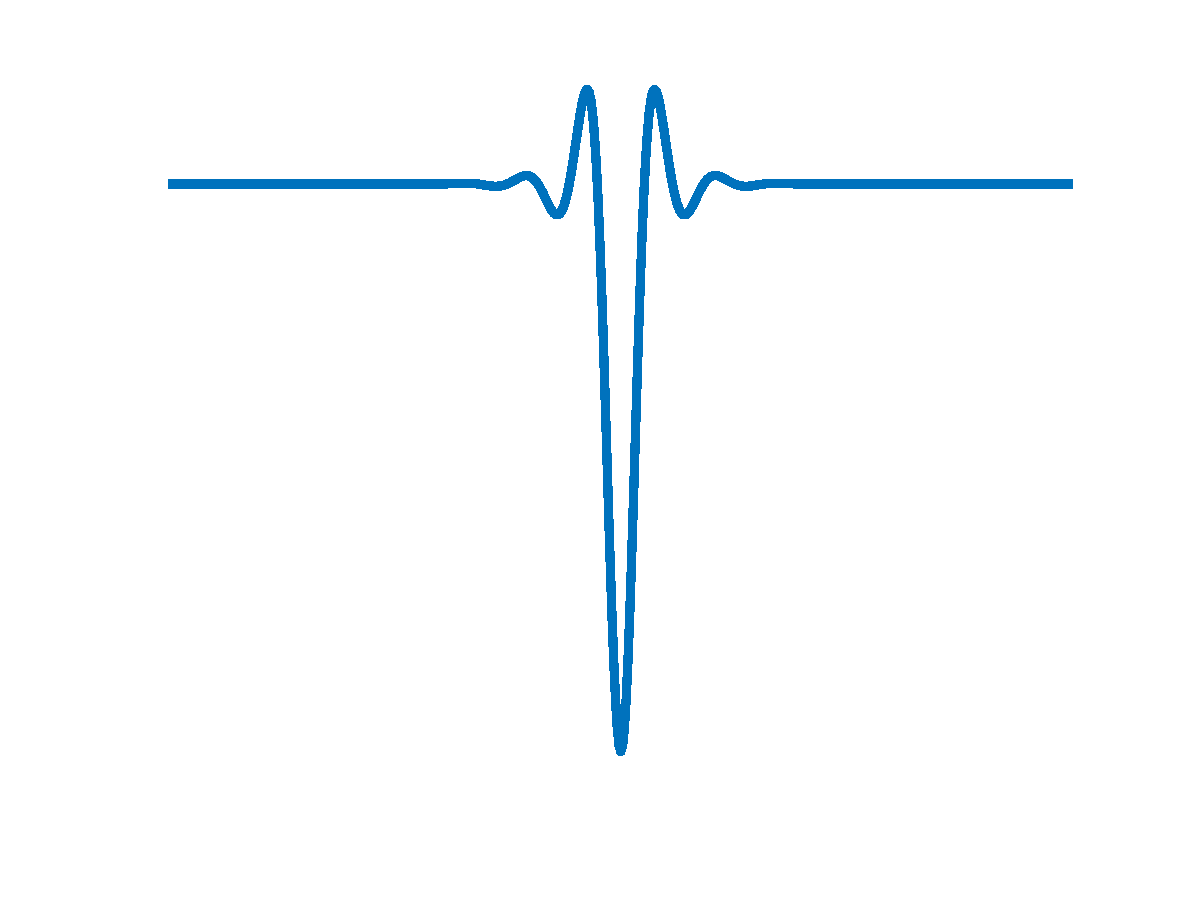
\includegraphics[width=5.25cm]{images/slidesingle12.eps}
          \includegraphics[width=5.25cm]{images/slidedouble12.eps}
          \end{center}
    \end{figure}

    Are multi-pulse solutions stable? 
    Visit Poster B30.


\end{frame}

\end{document}